\documentclass[tikz,border=10pt]{standalone}
\usepackage{amsmath}
\usepackage{tikz}
\usetikzlibrary{arrows.meta, positioning, calc, shapes.geometric}

\begin{document}
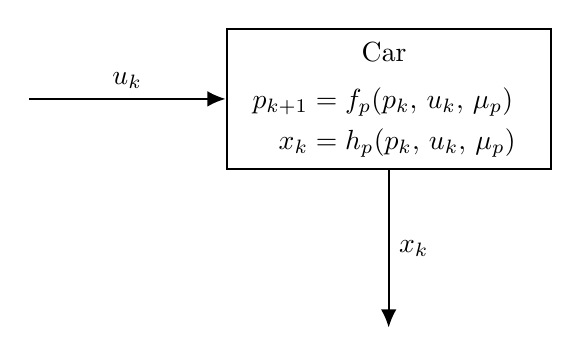
\begin{tikzpicture}[
  block/.style = {draw, thick, minimum height=3em, minimum width=6em, align=center},
  arrow/.style = {thick, -{Latex[width=2mm]}},
  node distance=2.5cm and 2.5cm
]

% Car (Plant) Block
\node[block] (siggen) {
  \begin{tabular}{c}
    Car \\[0.5em]
    $
    \begin{aligned}
      p_{k+1} &= f_p(p_k,\,u_k,\,\mu_p) \\
      x_k &= h_p(p_k,\,u_k,\,\mu_p)
    \end{aligned}
    $
  \end{tabular}
};

% Left input: u_k
\draw[arrow] ($(siggen.west)+(-2.5,0)$) --
  node[midway, above] {$u_k$} (siggen.west);

% Bottom output: x_k
\draw[arrow] (siggen.south) --
  node[midway, right] {$x_k$} ++(0,-2.0);

\end{tikzpicture}
\end{document}
